% Document class and parameters %
\documentclass[10pt,a4paper]{article}

% Document packages %
\usepackage{graphicx}
\usepackage{biblatex}
\usepackage{parskip}
\usepackage{listings}
\usepackage{caption}
\usepackage{subcaption}
\usepackage{amsmath}
\usepackage[most]{tcolorbox}


% Parameters %
\lstset{basicstyle=\ttfamily, breaklines = true, tabsize=2}
\graphicspath{{./Images/}}
\setlength{\parskip}{1em}

% Document Body %
\begin{document}
\begin{titlepage}
	\centering
	{\scshape\LARGE Imperial College London \par}
	\vspace{1cm}
	{\scshape\Large Mathematics: Year 1\par}
	\vspace{1.5cm}
	{\huge\bfseries Laplace Transform\par}
	\vspace{2cm}
	{\Large\ Xin Wang }
	\vfill
	{\large \today\par}
\end{titlepage}

\begin{abstract}
Laplace Transform methods play a important role Analysis and Design of engineering systems. Laplace
Transform is concerned with the systematic solution of ordinary differential equations with constant
coefficients.\par 
Mathematical transformations are
used to simplify solutions of problems by creating a new domain in which it is easier to handle the
problem. The results are then inverse-transformed to give the desired results in the original
domain. \par 
Laplace Transform is an example of \textbf{Integral Transforms} like Fourier Transforms. Laplace
Transforms turn \textit{differential equations} in time domain $t$ to \textit{algebraic equations} in
complex frequency domain $s$. Initial Conditions are essential in Laplace Transforms, making it
perfect for solving initial-value problems e.g. electrical circuits and mechanical vibrations.
\end{abstract}

\tableofcontents
\pagebreak

% Sections Body %
\section{Introduction}
Given a function defined uniquely on $0\leq t \leq \infty$, the Laplace transform is defined as: 
$$\mathcal{L}[f(t)]=\overline{f}(s)=\int_{\infty}^{0}e^{-st}*f(t)dt$$ where $s$ can be complex \par 
This definition shows that Laplace transform is a \textbf{one-sided transform} - it works on
$[0,\infty]$ unlike Fourier transform $[-\infty,\infty]$. This suits its purpose for solving
initial-value problems where a function switches on at $t=0$ and where $f(0)$ is defined. \par 

The inverse transform is defined as: 
$$f(t)=
     \mathcal{L}^{-1}[\hat{f}(s)]=\oint_C e^{st}*\overline{f}(s)\,ds$$
It is very difficult to evaluate inverse transforms (Bromwich integrals), rather a Library of
Transforms is defined and problems are broken down into those standard blocks.

\section{Library of Laplace Transforms}
\subsection{Functions}
 \begin{enumerate}
     \item Constant function - $f(t)=1$:
     \begin{tcolorbox}[breakable,colback=white,colframe=black,width=\dimexpr\textwidth+12mm\relax,enlarge left by=-6mm]
        \begin{equation*} 
            f(t)=1 \Leftrightarrow \overline{f}(s)=\frac{1}{s} 
        \end{equation*}
        where $\Re (s)>0$
     \end{tcolorbox}
     Proof: 
     \begin{equation*} 
        \begin{aligned}
            \overline{f}(s)&=\int_{0}^{\infty}e^{-s*t} dt 
            \\ &=\left[ \frac{e^{-s*t}}{s} \right]_0^\infty 
            \\ &= \frac{1}{s}
        \end{aligned}
     \end{equation*}

     \item Exponential function - $f(t)=e^{at}$:
     \begin{tcolorbox}[breakable,colback=white,colframe=black,width=\dimexpr\textwidth+12mm\relax,enlarge left by=-6mm]
        \begin{equation*} 
            f(t)=e^{at} \Leftrightarrow \overline{f}(s)=\frac{1}{s-a} 
        \end{equation*}
        where $\Re (s-a)>0$
     \end{tcolorbox}
     Proof: 
     \begin{equation*} 
        \begin{aligned}
            \overline{f}(s)&=\int_{0}^{\infty}e^{-(s-a)*t} dt 
            \\ &=\left[ \frac{e^{-(s-a)*t}}{s-a} \right]_0^\infty 
            \\ &= \frac{1}{s-a}
        \end{aligned}
     \end{equation*}

     \item Sine function - $f(t)=\sin(at)$:
     \begin{tcolorbox}[breakable,colback=white,colframe=black,width=\dimexpr\textwidth+12mm\relax,enlarge left by=-6mm]
        \begin{equation*} 
            f(t)=\sin (at) \Leftrightarrow \overline{f}(s)=\frac{a}{s^2+a^2} 
        \end{equation*}
        where $\Re (s)>0$
     \end{tcolorbox}
     Proof: 
     \begin{equation*} 
        \begin{aligned}
            \mathcal{L}(e^{iat})&=\int_{0}^{\infty}e^{-(s-ia)*t} dt \\
            &= \frac{1}{s-ia} \\
            &= \frac{s+ia}{s^2+a^2} \\ 
            &= \frac{a}{s^2+a^2}
        \end{aligned}
     \end{equation*}

     \item Cosine function - $f(t)=\cos(at)$:
     \begin{tcolorbox}[breakable,colback=white,colframe=black,width=\dimexpr\textwidth+12mm\relax,enlarge left by=-6mm]
        \begin{equation*} 
            f(t)=\cos (at) \Leftrightarrow \overline{f}(s)=\frac{s}{s^2+a^2} 
        \end{equation*}
        where $\Re (s)>0$
     \end{tcolorbox}
     Proof: 
     \begin{equation*} 
        \begin{aligned}
            \mathcal{L}(e^{iat})&=\int_{0}^{\infty}e^{-(s-ia)*t} dt \\
            &= \frac{1}{s-ia} \\
            &= \frac{s+ia}{s^2+a^2} \\
            &= \frac{s}{s^2+a^2}
        \end{aligned}
     \end{equation*}
     \pagebreak

     \item Polynomial function - $f(t)=t^n$:
     \begin{tcolorbox}[breakable,colback=white,colframe=black,width=\dimexpr\textwidth+12mm\relax,enlarge left by=-6mm]
        \begin{equation*} 
            f(t)=t^n \Leftrightarrow \overline{f}(s)=\frac{n!}{s^{n+1}} 
        \end{equation*}
        where $n\geq 0$ and $\Re (s)>0$
     \end{tcolorbox}
     Proof: 
     \begin{equation*} 
        \begin{aligned}
            \overline{f}(s)&=\int_{0}^{\infty}e^{-st}*t^n dt \\
            &= -\frac{1}{s}\int_{0}^{\infty}t^n d[e^{-st}] \\
            &= \frac{n}{s}\int_{0}^{\infty}e^{-st}*t^{n-1}dt \\
            &= \frac{n}{s}*\overline{f}(s)_{n-1}
        \end{aligned}
     \end{equation*}

     \item Heaviside function - $f(t)=H(t-t_0)$:
     \begin{tcolorbox}[breakable,colback=white,colframe=black,width=\dimexpr\textwidth+12mm\relax,enlarge left by=-6mm]
        \begin{equation*} 
        f(t)=H(t-t_0) \Leftrightarrow \overline{f}(s)=\frac{e^{-s*t_0}}{s}
        \end{equation*}
        where $\Re (s)>0$
     \end{tcolorbox}
     Proof: 
     \begin{equation*} 
        \begin{aligned}
            \mathcal{L}[H(t-t_0)]&=\int_{0}^{\infty}e^{-st}*H(t-t_0) dt \\
            &= \int_{t_0}^{\infty}e^{-st} dt \\
            &= \frac{e^{-s*t_0}}{s} 
        \end{aligned}
     \end{equation*}

     \item Dirac ($\delta$) function - $f(t)=\delta(t-t_0)$:
     \begin{tcolorbox}[breakable,colback=white,colframe=black,width=\dimexpr\textwidth+12mm\relax,enlarge left by=-6mm]
        \begin{equation*} 
        f(t)=\delta(t-t_0) \Leftrightarrow \overline{f}(s)=e^{-s*t_0}
        \end{equation*}
        where $t_0 \geq 0$
     \end{tcolorbox}
     Proof: 
     \begin{equation*} 
        \begin{aligned}
            \int_{0}^{\infty}e^{-s*t}*\delta(t-t_0) dt = \begin{cases}
                e^{-s*t_0}\; t_0\geq 0 \\
                0\; t_0<0
            \end{cases} 
        \end{aligned}
     \end{equation*}
 \end{enumerate}

 \pagebreak

 \subsection{Theorems}
 \begin{enumerate}
     \item Shift theorem:
     \begin{tcolorbox}[breakable,colback=white,colframe=black,width=\dimexpr\textwidth+12mm\relax,enlarge left by=-6mm]
        \begin{equation*} 
        \mathcal{L}[e^{a*t}*f(t)] \Leftrightarrow \overline{f}(s-a)
        \end{equation*}
        where $\Re(s-a)>0$
     \end{tcolorbox}
     Proof: 
     \begin{equation*} 
        \begin{aligned}
            \mathcal{L}[e^{a*t}*f(t)] &= \int_0^{\infty}e^{-(s-a)t}*f(t) dt \\
            &= \overline{f}(s-a)
        \end{aligned}
     \end{equation*}

     \item Second shift theorem:
     \begin{tcolorbox}[breakable,colback=white,colframe=black,width=\dimexpr\textwidth+12mm\relax,enlarge left by=-6mm]
        \begin{equation*} 
        \mathcal{L}[H(t-a)*f(t-a)] = e^{-sa}*\overline{f}(s)
        \end{equation*}
     \end{tcolorbox}
     Proof: Let $\tau = t-a$
     \begin{equation*} 
        \begin{aligned}
            \mathcal{L}[H(t-a)*f(t-a)] &= \int_0^{\infty}e^{-s*t}*H(t-a)*f(t-a) dt \\
            &= e^{-s*a} \int_{-a}^{\infty}e^{-s*\tau}*H(\tau)*f(\tau) d\tau \\
            &= e^{-s*a} \int_{0}^{\infty}e^{-s*\tau}*f(\tau) d\tau \\ 
            &= e^{-s*a}*\overline{f}(s)  
        \end{aligned}
     \end{equation*}
     \pagebreak
     \item Convolution theorem:
     \begin{tcolorbox}[breakable,colback=white,colframe=black,width=\dimexpr\textwidth+12mm\relax,enlarge left by=-6mm]
        \begin{equation*} 
        \mathcal{L}\{f\star g\} = \overline{f}(s)*\overline{g}(s)
        \end{equation*}
        where the convolution between two functions $f(t)$ and $g(t)$ is defined as:
        \begin{equation*} 
            f\star g = \int_0^tf(u)*g(t-u) du
        \end{equation*}
     \end{tcolorbox}
     Proof: 
     \begin{figure} [h!]
         \centering
         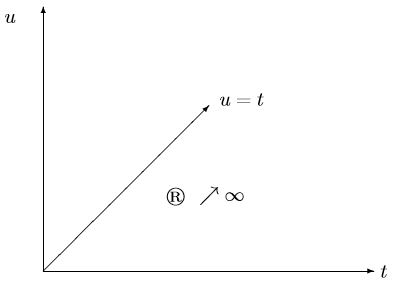
\includegraphics[scale=0.8]{Convolution.JPG}
         \caption{Region of integration obtained from original integral}
     \end{figure}
     \begin{equation*} 
        \begin{aligned} 
            \mathcal{L}\{f\star g\} &= \int_{0}^{\infty} e^{-s*t} \left( \int_{0}^{t} f(u)*g(u-t)du \right) dt \\
            &= \int_{0}^{\infty} \left( \int_{u}^{\infty} e^{-s*t}*g(t-u)dt \right)*f(u) du \\
            \text{Change of variables $\tau = t-u$} \\ 
            &= \int_{0}^{\infty} e^{-s*u} \left( \int_{\tau = 0}^{\tau = \infty} e^{-s*\tau}*g(\tau)d\tau \right) f(u) du \\
            &= \overline{f}(s)*\overline{g}(s)
        \end{aligned}
     \end{equation*}
     
     \item Integral theorem:
     \begin{tcolorbox}[breakable,colback=white,colframe=black,width=\dimexpr\textwidth+12mm\relax,enlarge left by=-6mm]
        \begin{equation*} 
        \mathcal{L}\left(\int_0^t f(u) du\right) = \frac{\overline{f}(s)}{s}
        \end{equation*}
     \end{tcolorbox}

     \item Derivative theorem:
     \begin{tcolorbox}[breakable,colback=white,colframe=black,width=\dimexpr\textwidth+12mm\relax,enlarge left by=-6mm]
        \begin{equation*} 
        \mathcal{L}[ f^{\prime}(t)] = s\overline{f}(s) - f(0)
        \end{equation*}
     \end{tcolorbox}
     Proof: 
     \begin{equation*} 
        \begin{aligned} 
            \mathcal{L}[\dot{f}]&=\int_0^{\infty}e^{-s*t}*\dot{f} dt \\
            &= \int_0^{\infty}e^{-s*t}df \\
            &= \left[e^{-s*t}*f(t)\right]_0^{\infty} + s\int_0^{\infty}e^{-s*t}*f dt \\
            &= s\overline{f}(s) - f(0)
        \end{aligned}
     \end{equation*}

     \item Second derivative theorem:
     \begin{tcolorbox}[breakable,colback=white,colframe=black,width=\dimexpr\textwidth+12mm\relax,enlarge left by=-6mm]
        \begin{equation*} 
        \mathcal{L}[ f^{\prime \prime}(t)] = s^2\overline{f}(s) - s\overline{f}(0) - f^{\prime}(0)
        \end{equation*}
     \end{tcolorbox}
     Proof: 
     \begin{equation*} 
        \begin{aligned} 
            \mathcal{L}[f^{\prime \prime}(t)]&=\int_0^{\infty}e^{-s*t}*\dot{f} dt \\
            &= \int_0^{\infty}e^{-s*t}df^{\prime} \\
            &= \left[e^{-s*t}*f^{\prime}(t)\right]_0^{\infty} + s\int_0^{\infty}e^{-s*t}*f^{\prime} dt \\
            &= s\mathcal{L}[f^{\prime}]-f^{\prime}(0) \\
            &= s^2\overline{f}(s) - s\overline{f}(0) - f^{\prime}(0)
        \end{aligned}
     \end{equation*}

 \end{enumerate}

 
\end{document}